\section{Pilot Study}
\label{sec:study}
\noindent Over the last year, we have designed, refined, and tested our measures and collected and begun analyzing pilot data from theses tests. Our results to date help to illustrate the power of our data collection approach and leave open many questions that we hope the proposed work will begin to answer. 

\subsection{Method}
\noindent
We focused our data collection on first-year students of a large public university as it allowed us to study students' experience in one of the challenging and critical periods of life.

\paragraph{Participants:}
\label{sec:study-participants}
We recruited 209 participants, of whom 176 stayed in the study through the end ($84\%$ retention rate). \tbl{tab:study-participants} provides further information about our sample at the beginning and end of the study. The age range of participants in the final sample was 18 - 23 years (M = 18.4, SD = 0.69).  We were particularly interested in sampling from among women in STEM, where gender discrimination is an ongoing problem \cite{johnson2018sexual}. We thus did snowball sampling for students enrolled in engineering majors. We oversampled women, minorities, and first generation students. 

\begin{table}[]
\small
\begin{tabular}{l|c|c|c|c|}
\cline{2-5}
& \multicolumn{2}{c|}{\begin{tabular}[c]{@{}c@{}}  \textbf{Completed Study}\end{tabular}} & \multicolumn{2}{c|}{\begin{tabular}[c]{@{}c@{}} \textbf{Dropped Out}\end{tabular}} \\ 
\cline{2-5} 
& \textbf{All (N=176)} & \textbf{Engineers (N=73)} & \textbf{All (N=33)} & \textbf{Engineers (N=11)} \\ 
\hline
\multicolumn{1}{|l|}{Women (64\%)} & 114 (54\%) & 41 (20\%) & 19 (9\%) & 7 (3\%)  \\
\hline
\multicolumn{1}{|l|}{\begin{tabular}[c]{@{}l@{}}URM (12\%) \end{tabular}} & 18 (9\%) & 15 (7\%) & 10 (5\%) & 5 (2\%) \\ \hline
\multicolumn{1}{|l|}{First Generation Students} & 51 (24\%) & 27 (13\%) & 11  (5\%) & 7 (3\%)  \\ \hline
\multicolumn{1}{|l|}{LGBTQIA+ (12\%)} & XX & XX & XXX & XX  \\
\hline 
\end{tabular}
\caption[UWEXP phase I - sample breakdown]{Sample breakdown in terms of gender and minority status. Percentages are  calculated out of 209 (the total number who began the study). Categories are non-independent. Of the 33 who dropped out, 13 did so before the break between quarters, and 20 before post questionnaire. URM refers to under-represented minorities (African-American students, Native American students, Latinx students, and Pacific Islander students).
}
\label{tab:study-participants}
\end{table}


\jm{need \%age of first gen students and percentagis for LGBTQIA+}


\paragraph{Surveys and Sensors:} Participants answered hour-long questionnaires about their life experiences, self regulation and coping skills, health behaviors, before and after the study (\textit{pre} and \textit{post} surveys). Participants  answered  twice weekly surveys abbout their affect, stress, and experiences of unfair treatment (EMA surveys).  For two weeks, we sent EMA surveys four times a day to get more detailed information. Of 209 participants, 176 (84\%)  completed the post questionnaire. The  compliance rate for EMA surveys was 85\%. 
location, activity, phone screen status, and call logs for incoming, outgoing and missed calls.
We gave participants a Fitbit~Flex~2, which records the number of steps and sleep status (\eg asleep or awake). \tbl{tab:study-sensors} summarizes the sensors we collected and details of their collection (\eg sampling rate). 

\begin{table}[]
\smaller
\begin{tabular}{p{1.5mm}|p{2.9cm}|l|p{9.3cm}|}
\cline{2-4}
 & \textbf{Measure}   & \textbf{Administration} & \textbf{Scales / Items Included in the Measure} \\ \hline
\multicolumn{1}{|c|}{\multirow{4}{*}{\vspace{-7mm}\rotatebox[origin=c]{90}{Pre or Post}}} & Social Experiences or Perceptions & pre, post & UCLA Loneliness(loneliness) [Russell \citeyear{Russell:1996}], 2-way SSS (social support) [Shakespeare-Finch \citeyear{Shakespeare:2011}]  \\ \cline{2-4} 
\multicolumn{1}{|c|}{} & \multirow{2}{*}{Stress \& Coping} & pre, post & MAAS [Brown, \citeyear{Brown:2003}], ERQ  (emotion regulation) [Gross \citeyear{Gross:2003}], PSS (stress) [Cohen \citeyear{Cohen:1983stress}], BRS  (resilience) [Smith \citeyear{Smith:2008}] \\ \cline{2-4} 
\multicolumn{1}{|c|}{} & Physical \& Mental Health% and Sleep 
& pre, post  & CHIPS [Cohen \citeyear{Cohen:1983positive}] (physical health), CES-D (depression) [Radloff \citeyear{Radloff:1977}], %RSQ \cite{Armey:2009}, 
STAI (anxiety) [Kabacoff \citeyear{Kabacoff:1997}]%, PSQI \cite{Buysse:1989} 
\\ \hline%\cline{2-4} 
\multicolumn{1}{|c|}{\multirow{6}{*}{\vspace{-7mm} \rotatebox[origin=c]{90}{EMA}}} & \multirow{2}{*}{Affect} & daily, weekly & Feeling \textit{Anxious}, \textit{depressed}, \textit{frustrated}, \textit{overwhelmed}, \textit{lonely}, \textit{happy}, and \textit{connected} on the scale of 1 (not at all) to 5 (extremely) \\ \cline{2-4} 
\multicolumn{1}{|c|}{} & \multirow{2}{*}{\textit{Unfair Treatment\dag}} %(exposure \& severity) 
& daily, weekly & Unfairly treated because of ancestry or national origins, gender, sexual orientation, intelligence, major, learning disability, education or income level, age, religion, physical disability, height, weight or other aspect of one's physical appearance\\ \hline
\end{tabular}
\caption{Measures in pre or post questionnaires and EMA surveys relevant to discriminaton analysis we present. The high level construct tapped by the measure is provided after the acronym and within parentheses. Predictor measures are italicized and marked with a cross (\dag). Other scales are considered as risk / protective factors (\ie resources) in our analysis.
}
\label{tab:study-surveys}
\end{table}

\begin{wrapfigure}{r}{0.5\textwidth}
\vspace{-.5cm}
    \centering
    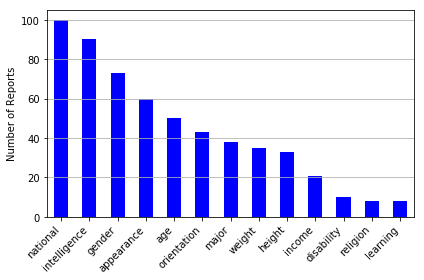
\includegraphics[width=3.3in]{img/discrimination_breakdown.png}
`    \caption[Unfair treatment type breakdown]{Breakdown of \numdiscriminationeventsfinal reports of unfair treatment by type. \textit{National}, \textit{Orientation}, and \textit{Learning} refer to ancestry or national origin, sexual orientation, and learning disability respectively. See \tbl{tab:study-surveys} for details of all categories. Participants were able to report multiple types of unfair treatment in each incident report.
}
    \label{fig:data-discrimination-breakdown}
\end{wrapfigure}

\paragraph{Measuring discrimination:} We used a single question, asked twice-weekly (daily on four separate weeks) to measure unfair treatment: ``Did you experience unfair treatment for any of the following reasons.'' This was followed by a list of possible reasons for unfair treatment ranging from ancestry / national origin, intelligence, and gender (the three most common) to religion, learning, and disability (the three least common, see \fig{fig:data-discrimination-breakdown}). \numdiscriminationevents distinct incidents of unfair treatment were reported in the duration of our study of which \numdiscriminationeventsfinal belong to participants whose sensor data is available for analysis. \fig{fig:data-discrimination-breakdown} shows the prevalence and breakdown of the reports of unfair treatment by category. We found that unfair treatment is more prevalent amongst women; 73\% of all reports of unfair treatment are reports from women. Contrary to our expectations, unfair treatment is equally prevalent in both engineering and non-engineering majors. 


\paragraph{Operationalizing Self Reported Variables }
In this preliminary study of the association between discrimination and behaviors, we consider all types of unfair treatment under one category of \textit{being discriminated}, which is used to drive two measures: \textit{exposure} (any report of unfair treatment qualifies) and \textit{severity} (ratio of total reports to total available responses, \ie number of times the question was answered over the course of the study). 
We also calculated measures of mental and physical health and behavior, both on \textit{pre/post} surveys and EMA surveys 
%Mental and psychological health  are taken from a simple question on momentary affect including anxiety, depression, frustrations, feeling overwhelmed, loneliness, happiness, and feeling connected 
(Table~\ref{tab:study-surveys}). 


\paragraph{Operaionalizing Behavioral Variables} Behaviors are operationalized as features calculated using the phone and Fitbit data.  We extracted behavior features from raw data obtained by AWARE using  the AWARE feature extraction library \citep{Chikersal:2019}. We calculate features daily and for four different parts of the day: night (12am-6am), morning (6am-12pm), afternoon (12pm-6pm), and evening (6pm-12am). We group the features into  the five categories that the literature suggests, described in Section~\ref{sec:data-features}. %Features captured were selected based on literature about reactions to discrimination (see Section~\ref{sec:back-mhealth}) and are summarized in \tbl{tab:data-features}.


\begin{table}[]
\centering
\smaller
\begin{tabular}{|l|l|l|l|p{5.5cm}|}
\hline
\textbf{Relevant Behavior}         & \textbf{Sensor} & \textbf{Source}        & \textbf{Sampling}            & \textbf{Information Collected}                                                 \\ \hline
\multirow{2}{*}{Physcial Activity} & Step            & Fitbit                 & 1 sample per min             & number of steps                                                                \\ \cline{2-5} 
                                   & Activity        & \multirow{4}{*}{AWARE} & 1 sample per 5 min           & Type of activity: walking, running, on bicycle, in vehicle, still, unknown     \\ \cline{1-2} \cline{4-5} 
\multirow{2}{*}{Phone Usage}                        & Screen          &                        & \multirow{2}{*}{event-based} & Screen status (locked, unlocked, off, and on) events                           \\ \cline{1-2} \cline{5-5} 
\multirow{2}{*}{Social Interactions} & Call            &                        &                              & Time and duration of incoming, outgoing, and missed calls                      \\ \cline{1-2} \cline{4-5} 
\multirow{2}{*}{Mobility}               & Location        &                        & 1 sample per 10 min          & GPS latitude, longitude, altitude                                              \\ \cline{2-2} \cline{4-5}
& Activity & & 1 sample per 5 min & Variety of activities \\ \hline
%Mobility               & Location        &                        & 1 sample per 10 min          & GPS latitude, longitude, altitude\\ \hline
\multirow{2}{*}{Sleep }                             & Sleep           & Fitbit                 & 1 sample per min             & Duration and onset of sleep, minutes to fall sleep, of awake, and after wakeup \\ \hline
\end{tabular}

\caption[Sensors]{Sensor data collected by AWARE and used in our analysis.}
\label{tab:study-sensors}
\end{table}

\paragraph{Analysis Approach}
%
We use hierarchical linear modeling (HLM) for analysis. HLM is an extension of linear regression for units (\eg individuals, schools, communities) with correlated/common features. %We use a two-level model in which individual participants, who were repeatedly sampled over time, are clustered within themselves.
%HLM allows for flexibility in how change over time is modeled such that these models can fit discontinuous and non-linear changes. Additionally, 
HLM models do not require that individuals report the same number of observations over time and thus can handle an unequal number of observations per person and uneven spacing between observations \cite{maas2005sufficient}. %\jm{ok but why not use HLM for both, or ridge regression for both?.} \yasaman{HLM stipulates hierarchy that does not exist in long-term data. as I have explaiend above, any form of regulaized model is inappropriate in examining the relationships between variables.}
%The data we use in our analysis can be considered in three main categories: 
Considering the inter-related nature of the variables and the sheer number of them, the behavior features considered as outcomes must be reduced to avoid an excessive number of comparisons that increase the chance of type I error. We used feature selection to reduce the size of the feature space before analysis. We select the top five metrics (when available) for each sensor for further analysis (\tbl{tab:analysis-short-behaviors}).


% \begin{table}[]
% \smaller
% \begin{tabular}{|p{5.6cm}|p{6.3cm}|p{3.3cm}|}
% \hline
% \multicolumn{3}{|c|}{\textbf{Daily Behaviors}} \\ \hline
% {\bf Mobility} & {\bf Social Interactions} & {\bf Sleep}\\
% \hline
% \# changes in activity             & \# calls                               & Length sleep       \\
% \# changes in activity (afternoon) & \# calls (evening)                     & Length main sleep  \\
% \# activities                      & \# incoming calls (evening)            & \# mins in bed        \\
% \# activities (afternoon)          & \# outgoing calls (evening)            & \# mins in bed  \\ 
% \# activities (evening)            & \# missed calls                        &  \ \ \ \ (main sleep)\\ \cline{2-3}
%  \% time in motion & {\bf Phone Usage} & {\bf Physical Activity}\\ \cline{2-3}
% \% time in motion       (afternoon)         & \# unlocks per minute (night)  &  Number of steps\\
%  Circadian movement                 & \# minutes interacting with phone      &  \\
% Circadian movement (afternoon)            & \# interactions with phone             &    \\
% \% time at home (night) & \# interactions with phone (morning)   &                       \\
%         & \# interactions with phone (afternoon) & \\ \hline
% \end{tabular}
% \caption[Daily features related to affect]{Daily behavior metrics selected by feature selection. These are grouped by categories of behaviors literature suggested as relevant to psychological distress. %\jm{maybe we should describe the variables better in a way that matches up with this?} \yasaman{this is unclear to me} 
% %\jm{what does this mean?} \yasaman{added clarifications}
% }
% \label{tab:analysis-short-behaviors}
% \end{table}
